% !TeX root = ../main-paper.tex
\section{Dataset}
\label{sec:dataset}

% Conventions nommage
% Dataset annoté à la main = "ground truth"
% ground truth aligné = "ner-reference"
% entrées pero aligné = "ner-pero"
% entrées tesseract alignées = "ner-tesseract"




%In this work, we  aim  at  producing  structured  spatio-temporal  data  from the information contained in the XIX\textsuperscript{th} century Parisian trade directories.
%To do this, it is therefore necessary to extract the text from the scans of the directories to be processed and to identify the entries in the various indexing lists used.
%Then, in each of these entries, the named entities they contain have to be extracted to produce structured spatio-temporal data representing the evolution over time of the people and businesses listed in these directories, their descriptions and their locations.
%Both of these extraction tasks require data to train and evaluate the OCR and NER approaches identified as potentially relevant: Tesseract and PERO OCR for the OCR task and Spacy and CamemBERT - pre-trained or fine-tuned - neural models for the NER task.

\subsection{A selection of Paris trade directories from 1798 to 1854}

The directories to be processed are stored in different libraries in Paris\footnote{\textcolor{green}{Citer les bibliothèques sources?} \joseph{est-ce nécessaire ici ? Est-ce que ça peut être dans une annexe ?}}. They have been scanned independently and with various levels of quality. Moreover, they cover a wide period and have been produced by different publishers and printers. Therefore, their contents, indexes, layouts, methods of printing, etc. may vary a lot from one directory to another (see Figure \ref{fig:directories}).


\begin{figure}[htb!]
	   \center{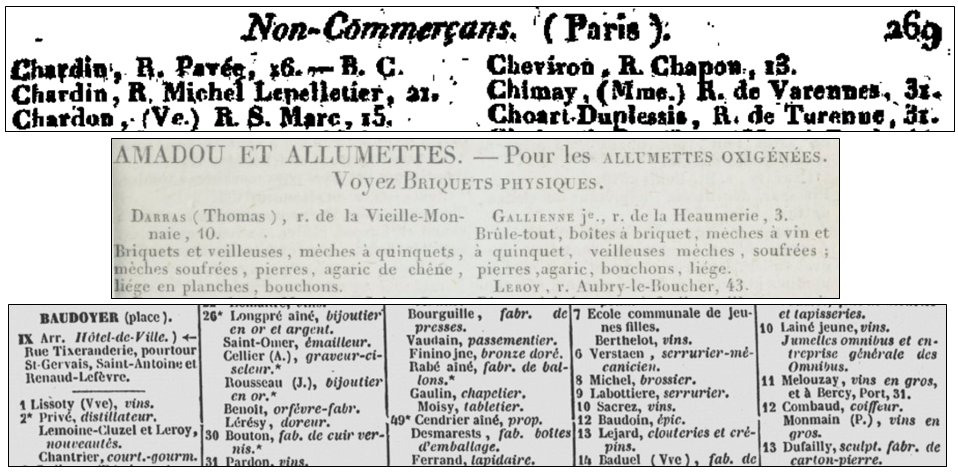
\includegraphics[width=0.9\textwidth]
	       {./images/DirectoryExcerpts2.png}}
	  \caption{\label{fig:directories} Examples of directory layouts and contents: 1) Duverneuil et La Tynna 1806 - index by name; 2) Deflandre 1828 - index by activity ; 3) Bottin 1851 - index by street name}
\end{figure}

For training as testing purposes, our groundtruth dataset must be as representative as possible of the diversity of the available directories. The Table \ref{tab:directories} lists the directories selected, their layout, the structure of their entries, and the number of annotated entries according to the considered index.

For example, the Didot directory of 1854 is organised according to three indexes: by name, by activity, and by street name. The structure of the following entry is characteristic of its index by name: "Batton (D.-A.) \scalerel*{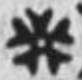
\includegraphics{./images/LH.png}}{H}, professeur au Conservatoire de musique et de déclamation, Saint-Georges, 47." This entry begins with a person's name, followed by the initials of their first name in parentheses.The symbol indicates that this person was awarded the Légion d'Honneur. The following part of this entry represents the person's activity,i.e. their profession, or social status, here "professor at the Conservatory of music and declamation". The street name and number where the person lives or carries out their activity are written at the end of the entry.

These pieces of information constituting the structure of the entries are the basic data that we want to extract, deduplicate and structure in order to build a spatio-temporal database of XIX\textsuperscript{th} century Parisian inhabitants and businesses. With the exception of some potentially wordy activity descriptions, they correspond to named entities. However, as Table \ref{tab:directories} shows, while most entries contain the same types of named entities, their order and the way they are written vary from one directory or index to another. To provide examples of each entry structure, pages from each type have thus been annotated\footnote{In this work, the street name index entries have not been included as they are very different from the others. The strategy to be adopted to process them without loss of quality for the NER model will be the subject of future work.}.


\subsection{Groundtruth data extraction}
\joseph{TODO: separate entry detection, OCR and NER stages explicitely}

First, the layout extraction and entry segmentation of the page are performed with a semi-automated system and
checked by a human. Afterward, an OCR system runs on the thumbnails of each segmented entry to extract its text. An
entry might span over multiple text lines but is always a single block. Thus, the most adapted mode is chosen when
the OCR system allows for the detection mode (e.g. the \emph{block} mode for \emph{Tesseract}). 

OCR: some basic charset normalization is performed after human annotation:
- remove annotation codes for glyphs which have no character in unicode
- alleviate some ambiguities in annotation rules (n° -> no, --- -> -, homogenize star and hand symbols allowed)


The annotated named entities are as follows:

\begin{itemize}
    \item PER: a person name or a business name, usually referred to as several person names. Firts names, initials, or civility mentions are included. E.g.: "Alibert (Prosper)", "Allamand frères et Hersent", "Heurtemotte (Vve)", etc.
    \item TITLE: an honorary title, either text, glyphs or a combination of the two. E.g: "O. \scalerel*{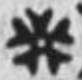
\includegraphics{./images/LH.png}}{H}" for "Officier de la Légion d'Honneur" or "\scalerel*{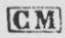
\includegraphics{./images/GMLondon.png}}{H}" to represent the Great Medal at the London exhibition.
    \item ACT: the profession or social status of a person summarized in the single concept of activity. E.g.: "horlogerie", "export en tous genres", "Conseiller d'Etat", "propriétaire".
    \item LOC: mostly street names ("r. de la Jussienne"), but may also be neighborhoods ("Marais du Temple") or any indirect spatial references ("au Palais Royal").
    \item CARDINAL: a street number, as part of an address ("16", "5 bis"), or a range of numbers (e.g. "23-25" or "5 à 9").
    \item FT: a geographic entity type, used to give more details on a location, e.g. "boutique", "atelier", "fab." or "dépôt".
\end{itemize}


Thus, the extracted corpus contains both the bounding boxes of directory entries, their exact text and the named entities they contain. It can therefore be used to train and improve the entry detection, OCR and NER tools.
% book, page, box, text_ocr, ner_xml (+uid within a page)

\subsection{Summary}
\joseph{TODO intégrer dans les sections avant ?}

\begin{verbatim}
[('<LOC>', 9709),
('<PER>', 8788),
('<CARDINAL>', 8747),
('<ACT>', 6472),
('<TITRE>', 483),
('<FT>', 43)]
\end{verbatim}
 
 valid ocr: 8765 entries
 
 valid ner (ref \& pero \& tess): 8341

\joseph{parler de l'étage d'extraction d'entrées qui est validé manuellement, et des quelques règles de simplification du charset pour homogénéiser entre les annotateurs / pallier des ambiguïtés dans les règles d'annotation (qu'on pourrait encore améliorer)}

TODO a word about the charset, and existence of glyphs unknown to the OCR

TODO average entry len (in char)

TODO average number of tags/entities per entry

TODO lists actual dataset content: set of entries. For each entry:
\begin{itemize*}
    \item ref to original book, page, region
    \item human transcription (OCR ref)
    \item human NER (NER ref)
    \item OCR produced by Pero OCR, Tesseract v4, Kraken (precise model used)
\end{itemize*}


\subsection{Metrics proposed}

\Cref{fig.protocol} depicts the evaluation protocol used to assess the OCR and NER systems. Two quality evaluations
are performed in the pipeline, respectively named \emph{OCR Q.A.} and \emph{NER Q.A.}.

First, the layout extraction and entry segmentation of the page are performed with a semi-automated system and
checked by a human. Afterward, an OCR system runs on the thumbnails of each segmented entry to extract its text. An
entry might span over multiple text lines but is always a single block. Thus, the most adapted mode is chosen when
the OCR system allows for the detection mode (e.g. the \emph{block} mode for \emph{Tesseract}). 

\textbf{OCR Q.A.} is performed after some text normalization of the OCR system outputs. Text normalization consists in
projecting Unicode characters onto the latin-1 \emph{charset} (whenever it makes sense) and removing extra symbols (hands,
crosses). Then, the predicted text is aligned with the reference text using standard tools from Stephen V. Rice's
thesis~\cite{santos.2019.wcmel,neudecker.2021.whdip} and the Character Error Rates (CER) are computed at the entry level
and at the global level. 

\begin{align}
\mathrm{CER} &=  \frac{\#Errors}{\text{Reference Text Length}} & & \mathrm{CER}_\mathrm{norm} =  \frac{\#Errors}{\text{Alignment Length}} 
\end{align}

In this benchmark, we consider 3 OCR systems well known for historical document analysis: Pero OCR, Tesseract, and Kraken. 


Next, a NER system extracts the named entities from the text of each entry output by the OCR and the \textbf{NER Q.A.}
is performed. The NER system outputs a text with tags that enclose the entities. To assess the quality of the entity
extraction, we rely on a technique similar as for the OCR evaluation. The predicted text is aligned with the reference
text and the tags are projected in the alignment. Then, the precision, recall, and f-measure (or f-score) are computed considering
only the exact matches between entities. Precision and recall are defined by equation (2); the f-measure is their harmonic mean.

\begin{align}
    \mathrm{precision} &= \frac{\text{\#exact matches}}{\text{\#entries in prediction}} & \mathrm{recall} &= \frac{\text{\#exact matches}}{\text{\#entries in reference}}
\end{align}


The whole process is illustrated on~\cref{fig.eval-ocr-ner}. The OCR text and the GOLD text are first aligned to
evaluate the OCR accuracy. As there are 11 mismatches over 56 aligned characters, the CER is thus 24\%. This alignment
is then used to back-project the GOLD tags to build the tagged NER reference string. Finally, the NER system runs on the
OCR text; its output is compared to the NER reference string. There is only 2 over 3 tags matching in the prediction (precision),
while only 2 over 4 entities are matched in the reference (recall). It follows an overall f-score of 0.4.

\begin{figure}[tb]
    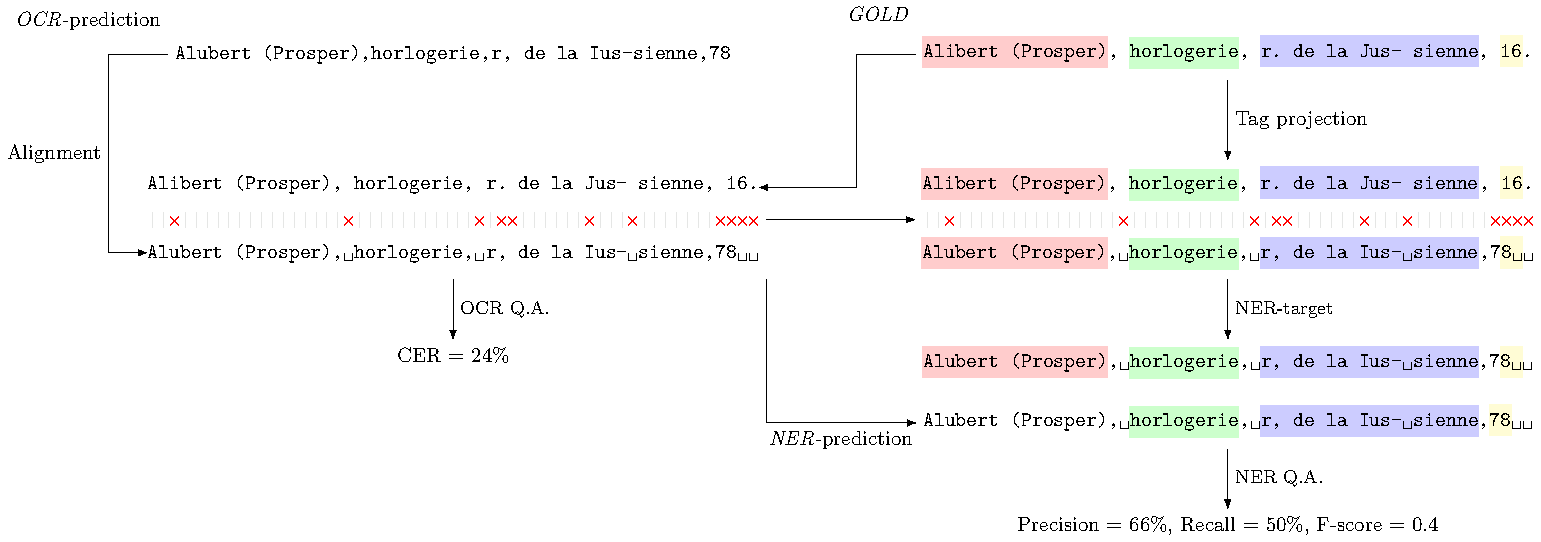
\includegraphics[width=\linewidth]{figs/eval-ocr-ner.pdf}
    \caption{OCR and NER evaluation protocol example.}
    \label{fig.eval-ocr-ner}
\end{figure}



\joseph{TODO expliquer qu'il faut faire la fusion des sous-datasets NER}

First and foremost, to make sure that the datasets contain the same entries a preprocessing step must be performed.
Indeed, entries where the OCR produced an empty string and those for which no entity could be projected from the gold reference text are ignored.
To overcome this problem we filter each dataset by keeping only the entries common to all.
At the cost of losing  5\% of the gold references entries, we thus have four new annotated datasets containing the exact same entries.

